\chapter{Tecnologias Web} % Main chapter title
\section{Html}
%--------------------------------------------------------
\subsection{Canvas}
En el nuevo estandar de HTML se define un nuevo elemento '<canvas>' el cual permite presentar graficos,graficos de juegos u otro tipo de elementos visuales sobre la marcha. El elemento lo denominamos lienzo que tiene forma rectangular en el cual utilizamos JavaScript para dibujar sobre él.
\\La coordenada (0,0) se encuentra en la esquina superior izquierda del lienzo.A lo largo del eje X, los valores aumentan hacia el borde derecho del lienzo.A lo largo del eje Y , los valores aumentan hacia el borde inferior del lienzo.punto inicial lo encontramos en el borde superior y los limites estan definidos por el ancho y el largo del lienzo.\ref{fig:canvas}
\begin{figure}[!h]
\begin{center}
   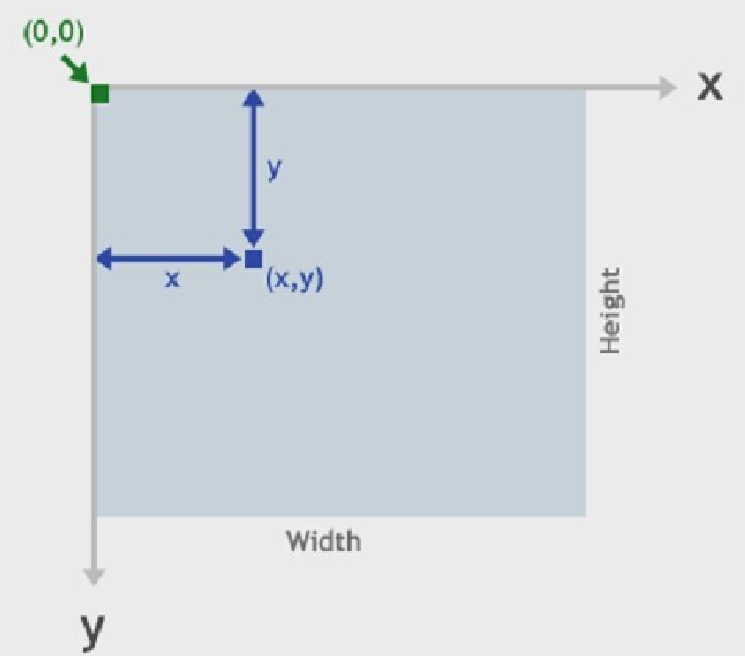
\includegraphics[width=0.4\linewidth, height=5cm]{Figures/canvas}
	\decoRule
	\caption[An Electron]{An electron (artist's impression).}
\label{fig:canvas}
\end{center}
\end{figure}
\\Los dibujos se reliazan a traves del contexto del elemento el cual permite trabajar/crear con los siguientes elementos
\begin{itemize}
\item Formas Simples 
\item Paths
\item Texto
\item Aplicar gradientes a lo elementos
\item Imagenes
\end{itemize}
%---------------------------------------------------------------------------
\subsection{API File}
Ofrece una forma estandar de interactuar  con archivos locales  a traves de la especificacion de esta API. Se puede utilizar para crear una vista previa en miniatura de imagenes mientras se envian al servidor o para permiitr que otra aplicacion guarde una referencia de un archivo cuando el usuario este sin conexion.
\begin{figure}[!h]
\begin{center}
    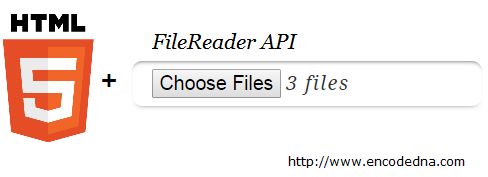
\includegraphics[width=0.6\linewidth]{Figures/fileReader}
	\decoRule
	\caption[An Electron]{An electron (artist's impression).}
\label{fig:canvas}
\end{center}
\end{figure}
\\Presente varios interfaces con los que es posible accedera a los archivos 
\begin{itemize}
\item \textit{File}: representa un archivo individual que proporciona informacion de lectura (nombre,tamaño del archivo,el tipo de MIME y una referencia al control del archivo).
\item \textit{FileList}: representa una secuencia de objetos File.
\item \textit{Blob}: permite fragmentar un archivo en intervalos de bytes.
\end{itemize}
 Cuando utilizamos las estructuras anteriores junto al interfaz de FileReader podemos leer un archivo de forma asincrona mendiante el control de eventos de JavaScript.
%-----------------------------------------------------------------------
\subsection{Media }
En cuanto al contenido multimedia HTML5 incluye  la etiqueta <video>  la que permite utilizar videos en la web.Antes para presentar el contenido multimedia se necesitaba  plugin's externos los cuales se encargaban de representa el contenido en la web uno de los mas conocidos es Flash.Tenia como inconveniente la necesidad del usario la instalacion del plugin pero con las nuevas etiquetas incorporadas en el estandar <audio> y <video> el navegador es ca
pas de reproducir el contenido de forma autonoma. 
\\La etiqueta <video>  permite tener varias fuentes del mismo archivo esto es debido a que los navegadores no son capaces de reproducir algunos formatos por lo que es recomendable dar varias fuentes para que el video pueda ser visualizado correctamente.
%--------------------- SUBSECCION ---------------------
\subsection{WebSockets}
Internet se ha creado en gran parte al paradigma cliente/servidor de HTTP. Un cliente carga una pagina web y no sucede nada hasta que el usuario haga un clic en un enlace o envie un formulario.
\\Hace algun tiempo se intento emplear tecnologias que permitan enviar datos al cliente en el momento que se detecta que hay nuevo datos disponibles como Comet si esto no funcionaba se empleaba Ajax. 
\\WebSocket no ofrece una conexión bidireccional entre el servidor y el navegador.La conexion se produce en tiempo real y se mantiene de forma permanentemente abierta hasta que cierre de forma explicita.
\begin{figure}[!h]
\centering
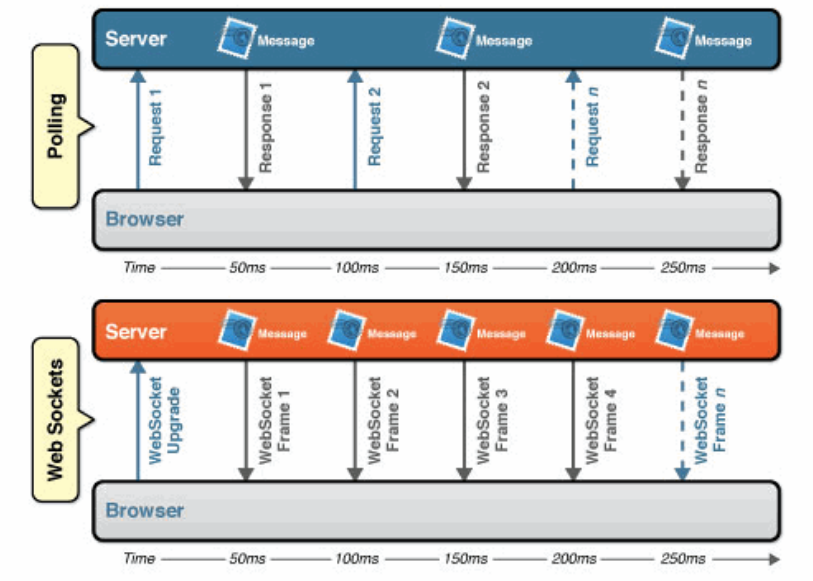
\includegraphics[width=0.5\linewidth]{Figures/websocketsDiag}
\decoRule
\caption[An Electron]{ComunnicacionWebRTC (artist's impression).}
\label{fig:ComunnicacionWebRTC}
\end{figure}
\\En el momento de disponer de un socket abierto, servidor puede enviar datos a todos los clientes conectados al socket , sin tener que crear y procesar peticiones como sucede con Ajax. Las ventaja que presenta esta API son las siguientes 
\begin{itemize}
\item Rendimiento y escalabilidad
\item Poca latencia ya que el canal siempre esta abierto y escuchando.
\end{itemize}
%--------------------------------------------------------------
\subsection{WebRTC}
Esta diseñada para permitir que las aplicaciones JS que permite crear conexiones en tiempo real con canales de audio, video y/o datos directamente entre usuarios a través de sus navegadores.
\begin{figure}[!h]
\centering
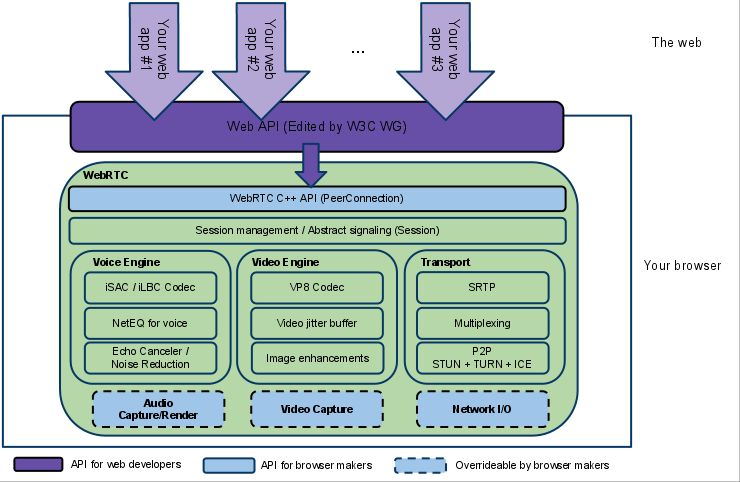
\includegraphics[width=0.5\linewidth]{Figures/webrtcdiagram}
\decoRule
\caption[An Electron]{ComunnicacionWebRTC (artist's impression).}
\label{fig:ComunnicacionWebRTC}
\end{figure}
La API se apoya en tres API
\begin{itemize}
\item GetUserMedia \\ Permite acceder a la cámara y micrófono de nuestro equipo.Para establecer una instancia  necesitamos pasar tres parámetros que son:  xxxx, una función de éxito que se activara cuando el usuario permita el acceso a los elementos y finalmente un función de fallo que muestra el motivo por el que ha fallado
\item RTCPeerConnection \\Se utiliza para comunicar el flujo de datos entre los navegadores pero para llevar acabo esta necesita un mecanismos de coordinación y control de los mensajes, es decir , un mecanismo de señalización.
De esta tarea no se encarga RTCPeerConnection sino que se puede utilizar métodos y mecanismos de señalización ya existentes. Se utiliza para intercambiar tres tipos de información: 
\begin{enumerate}
\item Mensajes de inicio de sesión
\item Configuración de red : peticiones a servidores STUN/TURN.
\item Características de los medios
\end{enumerate}
Como se puede apreciar este es el componente se encarga que la comunicación sea estable y eficiente, a continuación mostramos se presenta una imagen de la arquitectura de WebRTC y donde se puede apreciar el papel WebRTC.
\item DataChannel \\
\end{itemize}
%--------------------------------------------------------------------------------------
\subsection{LocalStorage}
El almacenamiento local persistente es una de las areas de interes que las aplicaciones web carecian.Historicamente, para las aplicaciones web se inventaron las cookies para el almacenamiento local persistentes de pequeñas cantidades de datos. Pero presentaba algunos  incovenientes:
\begin{itemize}
\item Se envian en todas las solicitudes HTTP, por lo que la aplicacion se ve ralentizada.
\item Los datos que se envian en la Cookie no estan cifrados.
\item El espacio de almacenamiento es alredodr de 4 KB que en ocaciones resulta insuficiente y logra un retraso considerable en la aplicacion.
\end{itemize}
Despues de varios intentos de dotar a la web de un almacenamiento local nativo, no fue hasta la aparicion de Html5 	quien lo consiguio.
\\Recibio del nombre LocalStorage mediante el cual las paginas web podian almacenar pares clave/valor localmente, dentro del  navegador web del cliente.Al igual que las cookies, los datos persistian incluso despúes de navegar fuera de la pagina web,cerrar el navegador pero estos no son transmitidos al servidor.
\\La compatibilidad de esta API en los distintos navegadores se presenta en la imagen ref 2.2
\begin{figure}[!h]
\centering
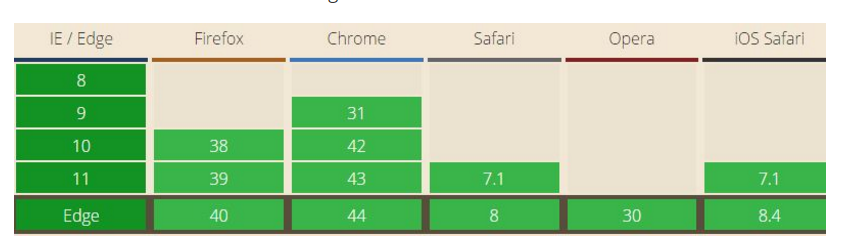
\includegraphics[width=0.6\linewidth]{Figures/compatibilidadLocalStorage}
\decoRule
\caption[An Electron]{ComunnicacionWebRTC (artist's impression).}
\label{fig:ComunnicacionWebRTC}
\end{figure}
%-------------------------------------------------------------------
\section{JavaScript}
La Web es un sistema Hipertexto, una cantidad de dimensiones gigantes de textos interrelacionados por medio de enlaces. En un principio, para diseñar este sistema de páginas con enlaces se pensó en un lenguaje que permitiese presentar cada una de estas informaciones junto con unos pequeños estilos, este lenguaje fue HTML. 
\\Conforme fue creciendo el Web y sus usos se fueron complicando por lo que se vio que HTML no era suficiente para realizar todas las acciones que se pueden llegar a necesitar en una página web. 
\\Al complicarse los sitios web, una de las primeras necesidades fue que las páginas respondiesen a las acciones del usuario, para desarrollar pequeñas funcionalidades más allá de los propios enlaces. El primer ayudante para cubrir las necesidades que estaban surgiendo fue Java, que es un lenguaje de propósito general, que había creado una manera de incrustar programas en páginas web a través de la tecnología de los Applets.La programación de Applets fue un gran avance y rompio la primera barrera del HTML al hacer posible la programación dentro de las páginas web.
\\Años depues se empezo a crear un lenguaje mas sencillo de trabajar dando lugar a Javacript. JavaScript es un lenguaje de programación utilizado para crear pequeños programas encargados de realizar acciones dentro del ámbito de una página web.Destaca por ser un lenguaje de programación bastante sencillo y pensado para hacer las cosas con rapidez.
\\Entre las acciones típicas que se pueden realizar  tenemos dos vertientes. Por un lado los efectos especiales sobre páginas web, para crear contenidos dinámicos , cambien de color o cualquier otro dinamismo. Por el otro, javascript nos permite ejecutar instrucciones como respuesta a las acciones del usuario, con lo que podemos crear páginas interactivas con programas como calculadoras, agendas, o tablas de cálculo.  
%---------------------------------------------------------------
\section{Jquery}
Se ha convertido rapidamente enun herramienta importane en el desarrollo del interfaz de una web. 
\\Se trata de una biblioteca rápida, pequeña y rica en funciones de JavaScript.Dentro de estas funciones se pueden destacar las siguientes:
\begin{itemize}
\item Recorrer y manipular el documento HTML
\item Manejo de eventos
\item Manejo de animaciones
\item Modificacion del estilo 
\item Ajax
\item Gran compatibilidad con los navegadores
\end{itemize}
 A parte de las funcionalidades descritas su ventaja es el acceso rapido y corto a los elementos comparado con el acceso tradicional.
%---------------------------------------------------------------
\section{NodeJs}
Nace en 2009 como respuesta a algunas necesidades encontradas a la hora de desarrollar sitios web, específicamente el caso de la concurrencia y la velocidad.Es un entorno JavaScript de lado de servidor que utiliza un modelo asíncrono y dirigido por eventos.
\subsubsection{Comparacion con Apache}
Apache crea un nuevo hilo por cada conexión cliente-servidor. Esto funciona bien para pocas conexiones, pero crear nuevos hilos es algo costoso, así como los cambios de contexto. Mientras que Node tiene  capacidad de mantener muchas conexiones abiertas y esperando.
\\Una aplicación para Node se programa sobre un solo hilo. Si en la aplicación existe una operación bloqueante (I/O por ejemplo), Node creará entonces otro hilo en segundo plano, pero no lo hará sistemáticamente por cada conexión como haría Apache. En teoría Node puede mantener tantas conexiones como número máximo de archivos descriptores (sockets) soportados por el sistema. Un inconveniente de Node es que debido a su arquitectura de usar sólo un hilo también que sólo puede usar una CPU. Un método para usar múltiples núcleos sería iniciar múltiples instancias de Node en el servidor y poner un balanceador de carga delante de ellos.
%---------------------------------------------------------------
\section{Django(FrameWork)}
Los desarrolladores que empleaban el modelo CGI para construir sus sitios web se dieron cuenta que tenian que construir paginas desde 0 y que muchas veces tenian cosas en comun por lo que tenian que refactorizar el contenido común entre las paginas lo que dio lugar a la creacion de framework.
\begin{figure}[!h]
\centering
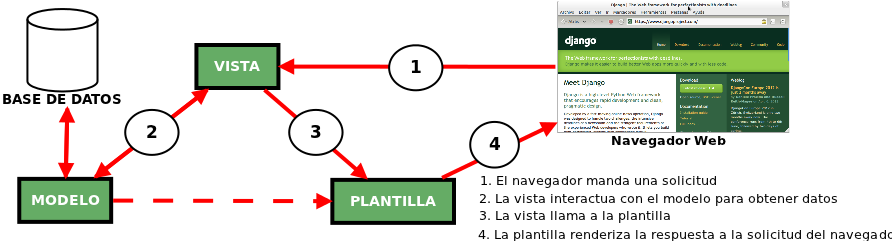
\includegraphics[width=0.8\linewidth]{Figures/esquemaDjango}
\decoRule
\caption[An Electron]{ComunnicacionWebRTC (artist's impression).}
\label{fig:ComunnicacionWebRTC}
\end{figure}
Normalmente un framework se basa en un patron de diseño denominado MVC a traves del cual se genera todo el contenido de la web. Un punto destacable es que el contenido se encuentra separado en tres partes segun su funcionamiento
\begin{itemize}
\item \textit{Models}:contiene  la descripcion de la base de datos y se define a traves de una clase de Python denominado  modelo.
\item \textit{View}:contienen toda la lógica de la pagina
\item \textit{Urls}: especifica que vista es llamada segun el patron URL
\item \textit{Template}:pantilla HTML que describe el diseño de la pagina
\end{itemize}
Con todos estos elementos nos aproximamos al diseño Modelo-Vista-Controlador. Una ventaja que presenta  es que poseen un acoplamiento debil entre si,es decir, cada pieza de la aplicacion Web que funciona sobre Django tiene un unico objetivo que al ser modificado no afecta a los otros .Ademas presenta un interfaz Admin a traves del cual se admistra el contenido de forma sencilla
